\documentclass[conference]{IEEEtran}

\usepackage[pdftex]{graphicx}
% \usepackage{amsmath}
% \usepackage{afterpage}
% \usepackage{wrapfig}
% \usepackage{tabularx}
% \usepackage{subfigure}
\usepackage{caption}
% \usepackage{tabu}
% \usepackage{booktabs}
% \usepackage{multicol}
% \usepackage{hyperref}

\hyphenation{op-tical net-works semi-conduc-tor}

\begin{document}

\title{DQM4HEP : A generic\\Data Quality Monitoring for High Energy Physics}

\author{

\IEEEauthorblockN{R\'emi \'Et\'e}
\IEEEauthorblockA{Univ, Lyon, Universit\'e Lyon 1, \\
CNRS/IN2P3, IPNL 4 rue E Fermi \\
69622, Villeurbanne CEDEX, France\\
Email: rete@ipnl.in2p3.fr}

\and

\IEEEauthorblockN{Antoine Pingault}
\IEEEauthorblockA{Ghent University, Department of Physics \\
and Astronomy Proeftuinstraat 86,\\
B-9000 Gent, Belgium\\
Email: antoine.pingault@ugent.be}

\and

\IEEEauthorblockN{Laurent Mirabito}
\IEEEauthorblockA{Univ, Lyon, Universit\'e Lyon 1, \\
CNRS/IN2P3, IPNL 4 rue E Fermi \\
69622, Villeurbanne CEDEX, France\\
Email: mirabito@ipnl.in2p3.fr}

}

\maketitle

\IEEEpeerreviewmaketitle

\section{Introduction}

With increasingly sophisticated devices, online data quality monitoring is of a significant importance for the detector and operation efficiency. Monitoring data is also a first step to a certification of the reliability of the recorded data for offline physics analyses. Experiments usually develop their event data model and file format to access and store their data. This dependency makes the monitoring systems even more specific for each experiment and leads to difficulties to adapt it for other ones.

With this in mind, a generic online data quality monitoring system has been developed without any assumption on the event data model and data type to treat. A dedicated implementation, based on the LCIO~\cite{LCIO} event data model for the Linear Collider collaboration was also developed. This implementation was put to real condition testing using a combined detector setup with the CALICE~\footnote{CAlorimeter for LInear Collider Experiment} Semi-Digital Hadronic CALorimeter (SDHCAL) and Silicon Tungsten Electronic Calorimeter (SiWECal) prototypes during test beam campaigns at CERN\footnote{Conseil Européen pour la Recherche Nucléaire}.

\section{Key points and software architecture}

The framework is designed to be run in separate processes and linked by TPC/IP using DIM\cite{dim1993distributed} and HTTP protocol using Mongoose\cite{MONGOOSE}. It is strongly based on a plugin system that allows some part of the software to be switched from one to another. This design enable the data serialization process to be encapsulated in plugins and loaded at run-time by the framework.

\begin{figure}[htbp]
  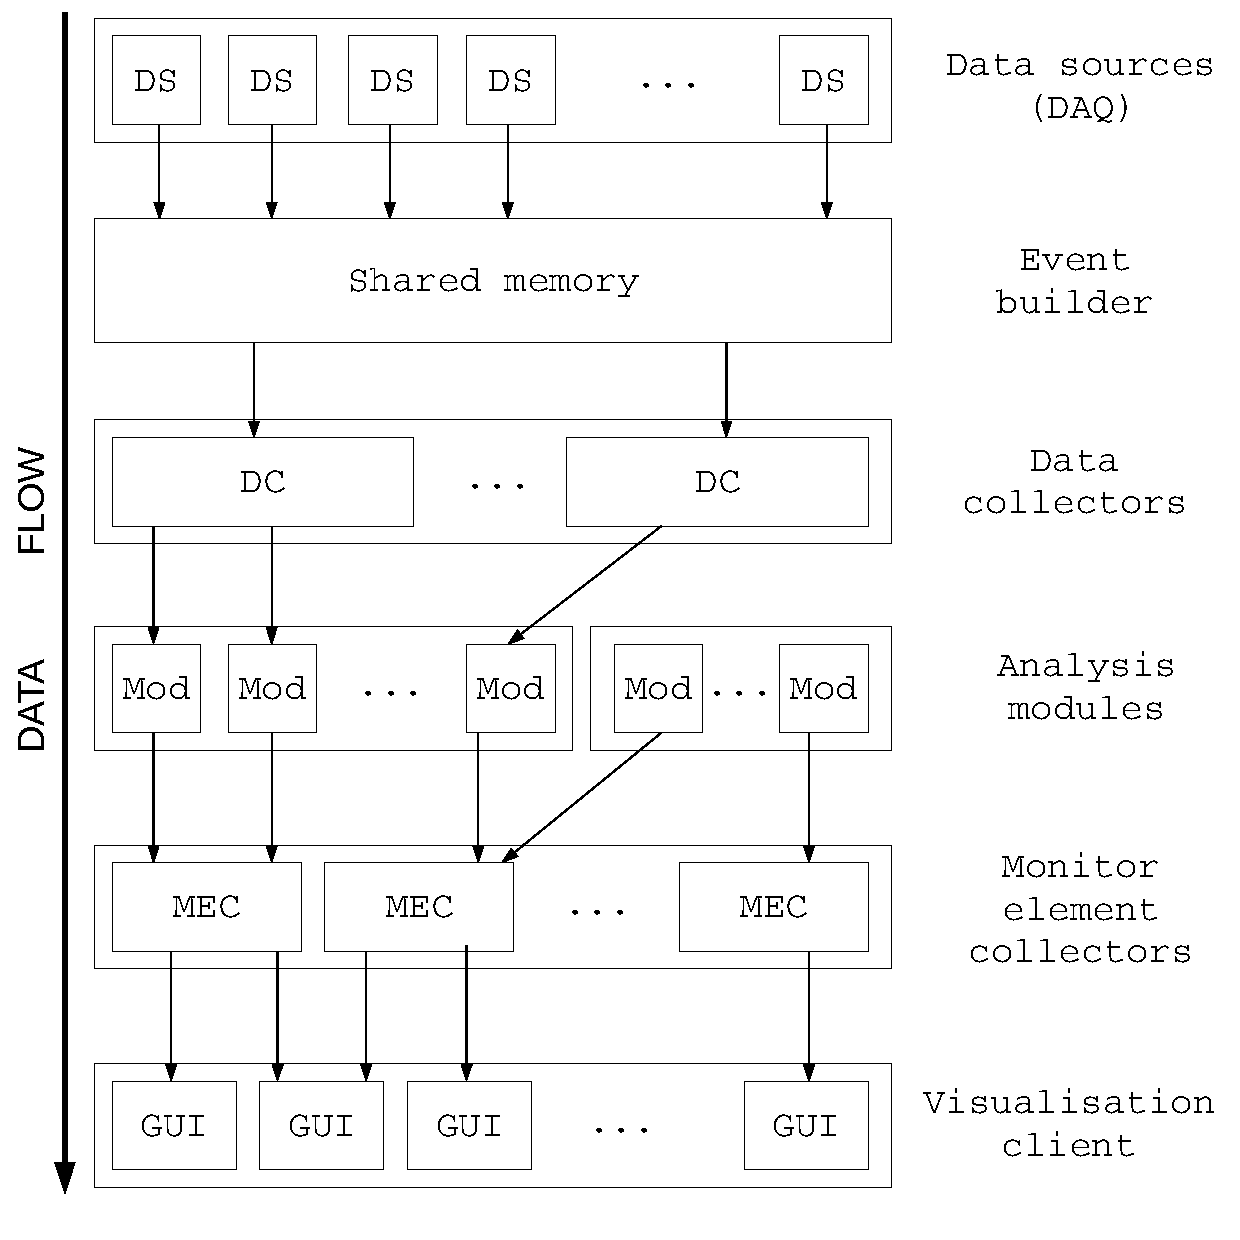
\includegraphics[width=\linewidth]{DQMWorkflow.pdf}
  \caption{\label{DQM_WORKFLOW}The monitoring framework data flow : from data sources to visualization}
\end{figure}

Fig. \ref{DQM_WORKFLOW} shows the monitoring framework data flow from incoming data sources to the client visualization computers. An important effort has been put on a generic interface to the data acquisition system and the development of an event builder. An independent DAQ process dumps the data sources content in the shared memory (shm) until a given limit in bytes is reached (set by the DAQ). In this way, a slow data treatment by the monitoring will not affect the data taking and writing to disk. Since the data structure is setup dependent, the implementation of the event builder becomes highly specific. The event building is encapsulated in series of \textit{shm processors} that convert data sources buffers into the user data structure. The whole reconstructed event is then serialized, dispatched across the network and stored into one or multiple data collector server applications.

Client interfaces are provided to either perform manual queries of collected data or work in update mode for which the data is directly forwarded on reception. User's online data analysis are also implemented as plugins in the system and steered using configuration files, increasing the modularity of the framework. They use a data collector client interface in update mode to receive and process data. 

The main purpose of the online data analysis is to reduce the initial amount of data to a few monitorable quantities, summarizing its quality and the status of the detection systems. Such quantities have been encapsulated in a unique interface called 'monitor elements' using ROOT \cite{ROOT}. An API is provided for the online analysis module to book and publish frequently these elements across the network. Published monitor elements are in their turn collected by server applications and distributed to clients, again, either on manual query or in update mode.

To visualize monitor elements from the collectors, a graphical user interface has been developed using the Qt \cite{QT} Gui toolkit. This interface can use multiple monitor element client interfaces to every available collectors on the network. The user can then display received \textit{monitor elements} in areas organized in tabs. Multiple configurations with different sets of monitor elements can be set-up at once. This allows for a quick overview of all the critical elements and variables needed for the good operation of the experiment.

\section{Implementation and tests}
Blablabla

\section{Conclusion}
Blablabla


\begin{thebibliography}{1}

% \bibitem{IEEEhowto:kopka}
% H.~Kopka and P.~W. Daly, \emph{A Guide to \LaTeX}, 3rd~ed.\hskip 1em plus
%   0.5em minus 0.4em\relax Harlow, England: Addison-Wesley, 1999.
  
\bibitem{QT}
Qt Company, \emph{\tt http://www.qt.io}, v4.7, 2016.

\bibitem{dim1993distributed}
C. Gaspar et al., \emph{DIM”, International Conference on Computing in High Energy and Nuclear Physics} (Padova,  Italy,
1-11 February 2000)

\bibitem{MONGOOSE}
Michael J Hammel. \emph{Mongoose: an embeddable web server in C}, Linux Journal, 2010(192):2, 2010.

\bibitem{ROOT}
I. Antcheva \textit{et al.}, Comput. Phys. Commun. \textbf{182}, 1384 (2011)

\end{thebibliography}




% 
%   \begin{abstract}
% 
% With increasingly sophisticated devices, online data quality monitoring is of a significant importance for the detector and operation efficiency. Monitoring data is also a first step to a certification of the reliability of the recorded data for offline physics analyses. Experiments usually develop their event data model and file format to access and store their data. This dependency makes the monitoring systems even more specific for each experiment and leads to difficulties to adapt it for other ones. 
% 
% With this in mind, a generic online data quality monitoring system has been developed without any assumption on the event data model and data type to treat. A specific implementation was developed based on the LCIO event data model for the Linear Collider collaboration and used to monitor the data taking of the CALICE SDHCAL and SiWECal prototypes during beam test compaigns at CERN. 
% 
% After introducing the key points of the framework, the software architecture is introduced with the key technical aspects. Details on the specific implementation for the ILC collaboration are presented. Finally, tests on the CALICE SDHCAL and SiWEcal combined detector setup using this implementation are described and used as proof of concept.
% 
% 
%   
%   
%   
% With increasingly sophisticated devices, online data quality monitoring is of a significant importance for the detector and operation efficiency. Monitoring data is also a first step to a certification of the reliability of the recorded data for offline physics analyses. The amount of data to treat in such experiments, becoming larger and larger, makes the monitoring systems more complex. To fastly evaluate data quality and detect anomalies during operation, automated procedures have to be set up. Experiments usually develop their event data model and file format to access and store their data. This dependency makes the monitoring systems even more specific for each experiment and leads to difficulties to adapt it for other ones. \\
% 
% With this in mind, a generic online data quality monitoring system has been developed without any assumption on the event data model and data type to treat. Different applications have been developed and designed to be run in separate processes linked using TPC/IP and HTTP protocols. An important effort has been put on a generic interface to the data acquisition system and the development of an event builder. The framework is strongly based on a plugin system that allows some part of the monitoring system to be switch from one to another. Thus, the data streaming is encapsulated in a plugin, loaded at runtime by the framework. Users online data analysis are also implemented as plugins in the system and steered using configuration files, increasing the modularity of the framework across the different possible experiments. Monitorable quantities have been encapsulated in a unique interface called 'monitor element' that analysis can book and publish frenquently accros the network. Distributed systems have been implemented for detector data and monitor elements in server applications to share available data and reduce the network load per process. \\
% 
% A specific implementation was developed based on the LCIO event data model for the Linear Collider collaboration and used to monitor the data taking of the CALICE SDHCAL prototype during beam test compaigns at CERN in real condition. A combined detector setup with the SiWECal prototype also maked the possibility to test the monitoring software with multiple data sources. \\
% 
% After introducing the key points of the framework, the software architecture is introduced with the key technical aspects. Details on the specific implementation for the ILC collaboration are presented. Finally, tests on the CALICE SDHCAL and SiWEcal combined detector setup using this implementation are described and used as proof of concept.
% 
%   \end{abstract}

  
\end{document}
